\begin{verbatim}
"""
Created on Mon Apr 15 19:43:04 2019

Updated on Wed Jan 29 10:18:09 2020

@author: created by Sowmya Myneni and updated by Dijiang Huang
"""
\end{verbatim}

\begin{verbatim}
'\nCreated on Mon Apr 15 19:43:04 2019\n\nUpdated on Wed Jan 29 10:18:09 2020\n\n@author: created by Sowmya Myneni and updated by Dijiang Huang\n'
\end{verbatim}

\begin{verbatim}
import matplotlib.pyplot as plt
import tensorflow as tf
print("Num GPUs Available:", len(tf.config.list_physical_devices('GPU')))
\end{verbatim}

\begin{verbatim}
Num GPUs Available: 0
\end{verbatim}

\begin{verbatim}
import os
import multiprocessing

# Number of logical CPUs
num_cores = multiprocessing.cpu_count()
print(f"Number of CPU cores available: {num_cores}")
\end{verbatim}

\begin{verbatim}
Number of CPU cores available: 12
\end{verbatim}

\begin{verbatim}
# Configure TensorFlow to use all available CPU cores
tf.config.threading.set_intra_op_parallelism_threads(0)  # Use all intra -operation threads
tf.config.threading.set_inter_op_parallelism_threads(0)  # Use all inter -operation threads
\end{verbatim}

\paragraph{FNN Sample SC}

\begin{verbatim}
########################################
# Part 1 - Data Pre -Processing
#######################################

# To load a dataset file in Python, you can use Pandas. Import pandas using the line below
import pandas as pd
# Import numpy to perform operations on the dataset
import numpy as np
\end{verbatim}

\subparagraph{Variable Setup}

\begin{verbatim}
# Variable Setup
# Available datasets: KDDTrain+.txt, KDDTest+.txt, etc. More read Data Set Introduction.html within the NSL -KDD dataset folder
# Type the training dataset file name in ''
#TrainingDataPath='NSL -KDD/'
#TrainingData='KDDTrain+_20Percent.txt'
# Batch Size
BatchSize=10
# Epohe Size
NumEpoch=10
\end{verbatim}

\subparagraph{Import Training Dataset}

\begin{verbatim}
# Import dataset.
# Dataset is given in TraningData variable You can replace it with the file 
# path such as “C:\Users\...\dataset.csv’. 
# The file can be a .txt as well. 
# If the dataset file has header, then keep header=0 otherwise use header=none
# reference: https://www.shanelynn.ie/select -pandas -dataframe -rows -and -columns -using -iloc -loc -and -ix/
dataset_train = pd.read_csv('Training -a1 -a2.csv', header=None)
\end{verbatim}

\begin{verbatim}
dataset_train.info()
\end{verbatim}

\begin{verbatim}
<class 'pandas.core.frame.DataFrame'>
RangeIndex: 124926 entries, 0 to 124925
Data columns (total 43 columns):
 #   Column  Non -Null Count   Dtype  
 - - -  - - - - - -  - - - - - - - - - - - - - -   - - - - -  
 0   0       124926 non -null  int64  
 1   1       124926 non -null  object 
 2   2       124926 non -null  object 
 3   3       124926 non -null  object 
 4   4       124926 non -null  int64  
 5   5       124926 non -null  int64  
 6   6       124926 non -null  int64  
 7   7       124926 non -null  int64  
 8   8       124926 non -null  int64  
 9   9       124926 non -null  int64  
 10  10      124926 non -null  int64  
 11  11      124926 non -null  int64  
 12  12      124926 non -null  int64  
 13  13      124926 non -null  int64  
 14  14      124926 non -null  int64  
 15  15      124926 non -null  int64  
 16  16      124926 non -null  int64  
 17  17      124926 non -null  int64  
 18  18      124926 non -null  int64  
 19  19      124926 non -null  int64  
 20  20      124926 non -null  int64  
 21  21      124926 non -null  int64  
 22  22      124926 non -null  int64  
 23  23      124926 non -null  int64  
 24  24      124926 non -null  float64
 25  25      124926 non -null  float64
 26  26      124926 non -null  float64
 27  27      124926 non -null  float64
 28  28      124926 non -null  float64
 29  29      124926 non -null  float64
 30  30      124926 non -null  float64
 31  31      124926 non -null  int64  
 32  32      124926 non -null  int64  
 33  33      124926 non -null  float64
 34  34      124926 non -null  float64
 35  35      124926 non -null  float64
 36  36      124926 non -null  float64
 37  37      124926 non -null  float64
 38  38      124926 non -null  float64
 39  39      124926 non -null  float64
 40  40      124926 non -null  float64
 41  41      124926 non -null  object 
 42  42      124926 non -null  int64  
dtypes: float64(15), int64(24), object(4)
memory usage: 41.0+ MB
\end{verbatim}

\begin{verbatim}
dataset_train.describe()
\end{verbatim}

\bigskip\noindent
\begin{tabular}{p{\dimexpr 0.045\linewidth-2\tabcolsep}p{\dimexpr 0.045\linewidth-2\tabcolsep}p{\dimexpr 0.045\linewidth-2\tabcolsep}p{\dimexpr 0.045\linewidth-2\tabcolsep}p{\dimexpr 0.045\linewidth-2\tabcolsep}p{\dimexpr 0.045\linewidth-2\tabcolsep}p{\dimexpr 0.045\linewidth-2\tabcolsep}p{\dimexpr 0.045\linewidth-2\tabcolsep}p{\dimexpr 0.045\linewidth-2\tabcolsep}p{\dimexpr 0.045\linewidth-2\tabcolsep}p{\dimexpr 0.045\linewidth-2\tabcolsep}p{\dimexpr 0.045\linewidth-2\tabcolsep}p{\dimexpr 0.045\linewidth-2\tabcolsep}p{\dimexpr 0.045\linewidth-2\tabcolsep}p{\dimexpr 0.045\linewidth-2\tabcolsep}p{\dimexpr 0.045\linewidth-2\tabcolsep}p{\dimexpr 0.045\linewidth-2\tabcolsep}p{\dimexpr 0.045\linewidth-2\tabcolsep}p{\dimexpr 0.045\linewidth-2\tabcolsep}p{\dimexpr 0.045\linewidth-2\tabcolsep}p{\dimexpr 0.045\linewidth-2\tabcolsep}p{\dimexpr 0.045\linewidth-2\tabcolsep}}
\toprule
 & 0 & 4 & 5 & 6 & 7 & 8 & 9 & 10 & 11 & 12 & ... & 32 & 33 & 34 & 35 & 36 & 37 & 38 & 39 & 40 & 42 \\
\hline
count & 124926.000000 & 1.249260e+05 & 1.249260e+05 & 124926.000000 & 124926.000000 & 124926.000000 & 124926.000000 & 124926.000000 & 124926.000000 & 124926.000000 & ... & 124926.000000 & 124926.000000 & 124926.000000 & 124926.000000 & 124926.000000 & 124926.000000 & 124926.000000 & 124926.000000 & 124926.000000 & 124926.000000 \\
\hline
mean & 284.472520 & 4.349730e+04 & 1.929105e+04 & 0.000200 & 0.022878 & 0.000080 & 0.139154 & 0.000776 & 0.391408 & 0.280470 & ... & 116.280150 & 0.519492 & 0.083460 & 0.144632 & 0.032099 & 0.286646 & 0.280689 & 0.119404 & 0.120862 & 19.587012 \\
\hline
std & 2607.625097 & 5.893836e+06 & 4.037690e+06 & 0.014145 & 0.254582 & 0.012653 & 1.706081 & 0.038056 & 0.488067 & 24.041762 & ... & 110.904962 & 0.449183 & 0.189509 & 0.304515 & 0.112446 & 0.445918 & 0.446814 & 0.307232 & 0.320212 & 2.078360 \\
\hline
min & 0.000000 & 0.000000e+00 & 0.000000e+00 & 0.000000 & 0.000000 & 0.000000 & 0.000000 & 0.000000 & 0.000000 & 0.000000 & ... & 0.000000 & 0.000000 & 0.000000 & 0.000000 & 0.000000 & 0.000000 & 0.000000 & 0.000000 & 0.000000 & 0.000000 \\
\hline
25\% & 0.000000 & 0.000000e+00 & 0.000000e+00 & 0.000000 & 0.000000 & 0.000000 & 0.000000 & 0.000000 & 0.000000 & 0.000000 & ... & 10.000000 & 0.050000 & 0.000000 & 0.000000 & 0.000000 & 0.000000 & 0.000000 & 0.000000 & 0.000000 & 18.000000 \\
\hline
50\% & 0.000000 & 4.400000e+01 & 0.000000e+00 & 0.000000 & 0.000000 & 0.000000 & 0.000000 & 0.000000 & 0.000000 & 0.000000 & ... & 64.000000 & 0.510000 & 0.030000 & 0.000000 & 0.000000 & 0.000000 & 0.000000 & 0.000000 & 0.000000 & 21.000000 \\
\hline
75\% & 0.000000 & 2.680000e+02 & 5.080000e+02 & 0.000000 & 0.000000 & 0.000000 & 0.000000 & 0.000000 & 1.000000 & 0.000000 & ... & 255.000000 & 1.000000 & 0.070000 & 0.060000 & 0.020000 & 1.000000 & 1.000000 & 0.000000 & 0.000000 & 21.000000 \\
\hline
max & 42908.000000 & 1.379964e+09 & 1.309937e+09 & 1.000000 & 3.000000 & 3.000000 & 77.000000 & 4.000000 & 1.000000 & 7479.000000 & ... & 255.000000 & 1.000000 & 1.000000 & 1.000000 & 1.000000 & 1.000000 & 1.000000 & 1.000000 & 1.000000 & 21.000000 \\
\hline
\bottomrule
\end{tabular}

\bigskip

8 rows $\times$ 39 columns

\begin{verbatim}
# Identify the column that contains the attack types
# Assuming the column with attack types is named based on the sample data ("neptune", "normal", etc.)
attack_column = dataset_train.columns[ -2]  # Second last column seems to have attack types

# Calculate the frequency of each attack type
attack_distribution = dataset_train[attack_column].value_counts()

plt.figure(figsize=(10, 6))
attack_distribution.plot(kind='bar', logy=True)
plt.title('A1 and A2 Training Dataset Distribution of Attack Types')
plt.xlabel('Attack Type')
plt.ylabel('Frequency')
plt.xticks(rotation=45)
plt.tight_layout()
plt.show()
\end{verbatim}

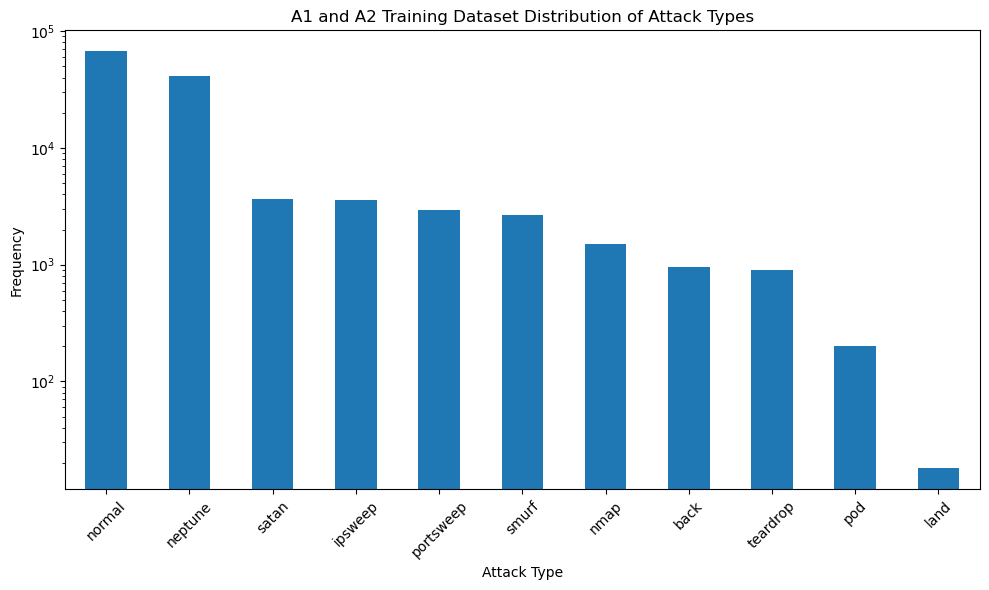
\includegraphics[width=0.7\linewidth]{files/19a134ccf8acdc940d3dff765098309e.png}

\begin{verbatim}
X_train = dataset_train.iloc[:, 0: -2].values
X_train
\end{verbatim}

\begin{verbatim}
array([[0, 'tcp', 'ftp_data', ..., 0.0, 0.05, 0.0],
       [0, 'udp', 'other', ..., 0.0, 0.0, 0.0],
       [0, 'tcp', 'private', ..., 1.0, 0.0, 0.0],
       ...,
       [0, 'tcp', 'smtp', ..., 0.0, 0.01, 0.0],
       [0, 'tcp', 'klogin', ..., 1.0, 0.0, 0.0],
       [0, 'tcp', 'ftp_data', ..., 0.0, 0.0, 0.0]], dtype=object)
\end{verbatim}

\begin{verbatim}
X_train.shape
\end{verbatim}

\begin{verbatim}
(124926, 41)
\end{verbatim}

\begin{verbatim}
label_column_train = dataset_train.iloc[:, -2].values
label_column_train
\end{verbatim}

\begin{verbatim}
array(['normal', 'normal', 'neptune', ..., 'normal', 'neptune', 'normal'],
      dtype=object)
\end{verbatim}

\begin{verbatim}
y_train = []
for i in range(len(label_column_train)):
    if label_column_train[i] == 'normal':
        y_train.append(0)
    else:
        y_train.append(1)

# Convert list to array
y_train = np.array(y_train)
\end{verbatim}

\begin{verbatim}
y_train
\end{verbatim}

\begin{verbatim}
array([0, 0, 1, ..., 0, 1, 0])
\end{verbatim}

\begin{verbatim}
y_train.shape
\end{verbatim}

\begin{verbatim}
(124926,)
\end{verbatim}

\subparagraph{Import Testing Dataset}

\begin{verbatim}
# Import dataset.
# Dataset is given in TraningData variable You can replace it with the file 
# path such as “C:\Users\...\dataset.csv’. 
# The file can be a .txt as well. 
# If the dataset file has header, then keep header=0 otherwise use header=none
# reference: https://www.shanelynn.ie/select -pandas -dataframe -rows -and -columns -using -iloc -loc -and -ix/
dataset_test = pd.read_csv('Testing -a1 -a2 -a3.csv', header=None)
\end{verbatim}

\begin{verbatim}
dataset_test.info()
\end{verbatim}

\begin{verbatim}
<class 'pandas.core.frame.DataFrame'>
RangeIndex: 19659 entries, 0 to 19658
Data columns (total 43 columns):
 #   Column  Non -Null Count  Dtype  
 - - -  - - - - - -  - - - - - - - - - - - - - -  - - - - -  
 0   0       19659 non -null  int64  
 1   1       19659 non -null  object 
 2   2       19659 non -null  object 
 3   3       19659 non -null  object 
 4   4       19659 non -null  int64  
 5   5       19659 non -null  int64  
 6   6       19659 non -null  int64  
 7   7       19659 non -null  int64  
 8   8       19659 non -null  int64  
 9   9       19659 non -null  int64  
 10  10      19659 non -null  int64  
 11  11      19659 non -null  int64  
 12  12      19659 non -null  int64  
 13  13      19659 non -null  int64  
 14  14      19659 non -null  int64  
 15  15      19659 non -null  int64  
 16  16      19659 non -null  int64  
 17  17      19659 non -null  int64  
 18  18      19659 non -null  int64  
 19  19      19659 non -null  int64  
 20  20      19659 non -null  int64  
 21  21      19659 non -null  int64  
 22  22      19659 non -null  int64  
 23  23      19659 non -null  int64  
 24  24      19659 non -null  float64
 25  25      19659 non -null  float64
 26  26      19659 non -null  float64
 27  27      19659 non -null  float64
 28  28      19659 non -null  float64
 29  29      19659 non -null  float64
 30  30      19659 non -null  float64
 31  31      19659 non -null  int64  
 32  32      19659 non -null  int64  
 33  33      19659 non -null  float64
 34  34      19659 non -null  float64
 35  35      19659 non -null  float64
 36  36      19659 non -null  float64
 37  37      19659 non -null  float64
 38  38      19659 non -null  float64
 39  39      19659 non -null  float64
 40  40      19659 non -null  float64
 41  41      19659 non -null  object 
 42  42      19659 non -null  int64  
dtypes: float64(15), int64(24), object(4)
memory usage: 6.4+ MB
\end{verbatim}

\begin{verbatim}
dataset_test.describe()
\end{verbatim}

\bigskip\noindent
\begin{tabular}{p{\dimexpr 0.045\linewidth-2\tabcolsep}p{\dimexpr 0.045\linewidth-2\tabcolsep}p{\dimexpr 0.045\linewidth-2\tabcolsep}p{\dimexpr 0.045\linewidth-2\tabcolsep}p{\dimexpr 0.045\linewidth-2\tabcolsep}p{\dimexpr 0.045\linewidth-2\tabcolsep}p{\dimexpr 0.045\linewidth-2\tabcolsep}p{\dimexpr 0.045\linewidth-2\tabcolsep}p{\dimexpr 0.045\linewidth-2\tabcolsep}p{\dimexpr 0.045\linewidth-2\tabcolsep}p{\dimexpr 0.045\linewidth-2\tabcolsep}p{\dimexpr 0.045\linewidth-2\tabcolsep}p{\dimexpr 0.045\linewidth-2\tabcolsep}p{\dimexpr 0.045\linewidth-2\tabcolsep}p{\dimexpr 0.045\linewidth-2\tabcolsep}p{\dimexpr 0.045\linewidth-2\tabcolsep}p{\dimexpr 0.045\linewidth-2\tabcolsep}p{\dimexpr 0.045\linewidth-2\tabcolsep}p{\dimexpr 0.045\linewidth-2\tabcolsep}p{\dimexpr 0.045\linewidth-2\tabcolsep}p{\dimexpr 0.045\linewidth-2\tabcolsep}p{\dimexpr 0.045\linewidth-2\tabcolsep}}
\toprule
 & 0 & 4 & 5 & 6 & 7 & 8 & 9 & 10 & 11 & 12 & ... & 32 & 33 & 34 & 35 & 36 & 37 & 38 & 39 & 40 & 42 \\
\hline
count & 19659.000000 & 1.965900e+04 & 1.965900e+04 & 19659.000000 & 19659.000000 & 19659.000000 & 19659.000000 & 19659.000000 & 19659.000000 & 19659.000000 & ... & 19659.000000 & 19659.000000 & 19659.000000 & 19659.000000 & 19659.000000 & 19659.000000 & 19659.000000 & 19659.000000 & 19659.000000 & 19659.000000 \\
\hline
mean & 236.416145 & 3.805797e+03 & 2.248116e+03 & 0.000356 & 0.009665 & 0.000763 & 0.066077 & 0.000712 & 0.441630 & 0.135612 & ... & 143.510657 & 0.598606 & 0.094687 & 0.130786 & 0.018738 & 0.110247 & 0.113759 & 0.259291 & 0.252741 & 18.892110 \\
\hline
std & 1447.471201 & 6.099660e+04 & 2.223105e+04 & 0.018867 & 0.152665 & 0.038401 & 0.937110 & 0.040340 & 0.496594 & 7.783397 & ... & 112.924502 & 0.444168 & 0.227570 & 0.302832 & 0.086176 & 0.288794 & 0.299062 & 0.403418 & 0.416891 & 3.357874 \\
\hline
min & 0.000000 & 0.000000e+00 & 0.000000e+00 & 0.000000 & 0.000000 & 0.000000 & 0.000000 & 0.000000 & 0.000000 & 0.000000 & ... & 0.000000 & 0.000000 & 0.000000 & 0.000000 & 0.000000 & 0.000000 & 0.000000 & 0.000000 & 0.000000 & 0.000000 \\
\hline
25\% & 0.000000 & 0.000000e+00 & 0.000000e+00 & 0.000000 & 0.000000 & 0.000000 & 0.000000 & 0.000000 & 0.000000 & 0.000000 & ... & 14.000000 & 0.060000 & 0.000000 & 0.000000 & 0.000000 & 0.000000 & 0.000000 & 0.000000 & 0.000000 & 18.000000 \\
\hline
50\% & 0.000000 & 5.500000e+01 & 4.400000e+01 & 0.000000 & 0.000000 & 0.000000 & 0.000000 & 0.000000 & 0.000000 & 0.000000 & ... & 190.000000 & 0.950000 & 0.010000 & 0.000000 & 0.000000 & 0.000000 & 0.000000 & 0.000000 & 0.000000 & 21.000000 \\
\hline
75\% & 0.000000 & 2.970000e+02 & 8.905000e+02 & 0.000000 & 0.000000 & 0.000000 & 0.000000 & 0.000000 & 1.000000 & 0.000000 & ... & 255.000000 & 1.000000 & 0.060000 & 0.030000 & 0.010000 & 0.000000 & 0.000000 & 0.570000 & 0.530000 & 21.000000 \\
\hline
max & 54451.000000 & 6.291668e+06 & 1.345927e+06 & 1.000000 & 3.000000 & 3.000000 & 101.000000 & 3.000000 & 1.000000 & 796.000000 & ... & 255.000000 & 1.000000 & 1.000000 & 1.000000 & 1.000000 & 1.000000 & 1.000000 & 1.000000 & 1.000000 & 21.000000 \\
\hline
\bottomrule
\end{tabular}

\bigskip

8 rows $\times$ 39 columns

\begin{verbatim}
# Identify the column that contains the attack types
# Assuming the column with attack types is named based on the sample data ("neptune", "normal", etc.)
attack_column = dataset_test.columns[ -2]  # Second last column seems to have attack types

# Calculate the frequency of each attack type
attack_distribution = dataset_test[attack_column].value_counts()

plt.figure(figsize=(10, 6))
attack_distribution.plot(kind='bar', logy=True)
plt.title('A1, A2 and A3 Testing Dataset Distribution of Attack Types')
plt.xlabel('Attack Type')
plt.ylabel('Frequency')
plt.xticks(rotation=45)
plt.tight_layout()
plt.show()
\end{verbatim}

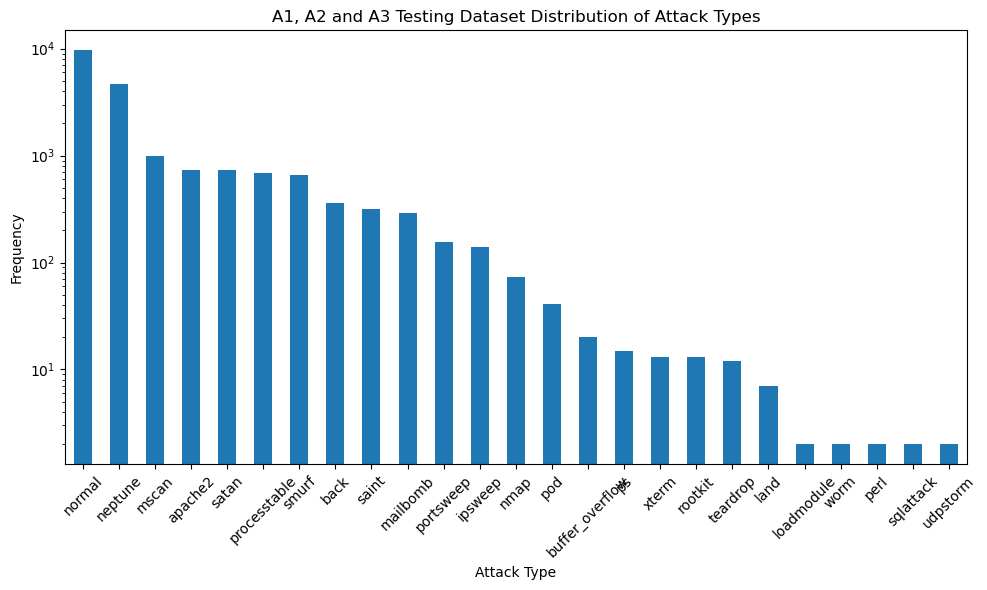
\includegraphics[width=0.7\linewidth]{files/5190bd8d6a86e7ec2e42669e7bf06af7.png}

\begin{verbatim}
X_test = dataset_test.iloc[:, 0: -2].values
X_test
\end{verbatim}

\begin{verbatim}
array([[0, 'tcp', 'private', ..., 0.0, 1.0, 1.0],
       [0, 'tcp', 'private', ..., 0.0, 1.0, 1.0],
       [2, 'tcp', 'ftp_data', ..., 0.0, 0.0, 0.0],
       ...,
       [0, 'tcp', 'http', ..., 0.0, 0.07, 0.07],
       [0, 'udp', 'domain_u', ..., 0.0, 0.0, 0.0],
       [0, 'tcp', 'sunrpc', ..., 0.0, 0.44, 1.0]], dtype=object)
\end{verbatim}

\begin{verbatim}
X_test.shape
\end{verbatim}

\begin{verbatim}
(19659, 41)
\end{verbatim}

\begin{verbatim}
label_column_test = dataset_test.iloc[:, -2].values
label_column_test
\end{verbatim}

\begin{verbatim}
array(['neptune', 'neptune', 'normal', ..., 'back', 'normal', 'mscan'],
      dtype=object)
\end{verbatim}

\begin{verbatim}
y_test = []
for i in range(len(label_column_test)):
    if label_column_test[i] == 'normal':
        y_test.append(0)
    else:
        y_test.append(1)

# Convert list to array
y_test = np.array(y_test)
\end{verbatim}

\begin{verbatim}
y_test
\end{verbatim}

\begin{verbatim}
array([1, 1, 0, ..., 1, 0, 1])
\end{verbatim}

\subparagraph{Encoding categorical data (convert letters/words in numbers)}

\begin{verbatim}
# The following code work Python 3.7 or newer
from sklearn.preprocessing import OneHotEncoder
from sklearn.compose import ColumnTransformer
ct = ColumnTransformer(
     # The column numbers to be transformed ([1, 2, 3] represents three columns to be transferred)
    [('one_hot_encoder', OneHotEncoder(handle_unknown='ignore'), [1,2,3])],
    # Leave the rest of the columns untouched
    remainder='passthrough'
)
X_train = np.array(ct.fit_transform(X_train), dtype=np.float64)
X_test  = np.array(ct.transform(X_test) , dtype=np.float64)
\end{verbatim}

\begin{verbatim}
X_train
\end{verbatim}

\begin{verbatim}
array([[0.  , 1.  , 0.  , ..., 0.  , 0.05, 0.  ],
       [0.  , 0.  , 1.  , ..., 0.  , 0.  , 0.  ],
       [0.  , 1.  , 0.  , ..., 1.  , 0.  , 0.  ],
       ...,
       [0.  , 1.  , 0.  , ..., 0.  , 0.01, 0.  ],
       [0.  , 1.  , 0.  , ..., 1.  , 0.  , 0.  ],
       [0.  , 1.  , 0.  , ..., 0.  , 0.  , 0.  ]])
\end{verbatim}

\begin{verbatim}
X_train[0]
\end{verbatim}

\begin{verbatim}
array([0.00e+00, 1.00e+00, 0.00e+00, 0.00e+00, 0.00e+00, 0.00e+00,
       0.00e+00, 0.00e+00, 0.00e+00, 0.00e+00, 0.00e+00, 0.00e+00,
       0.00e+00, 0.00e+00, 0.00e+00, 0.00e+00, 0.00e+00, 0.00e+00,
       0.00e+00, 0.00e+00, 0.00e+00, 0.00e+00, 0.00e+00, 1.00e+00,
       0.00e+00, 0.00e+00, 0.00e+00, 0.00e+00, 0.00e+00, 0.00e+00,
       0.00e+00, 0.00e+00, 0.00e+00, 0.00e+00, 0.00e+00, 0.00e+00,
       0.00e+00, 0.00e+00, 0.00e+00, 0.00e+00, 0.00e+00, 0.00e+00,
       0.00e+00, 0.00e+00, 0.00e+00, 0.00e+00, 0.00e+00, 0.00e+00,
       0.00e+00, 0.00e+00, 0.00e+00, 0.00e+00, 0.00e+00, 0.00e+00,
       0.00e+00, 0.00e+00, 0.00e+00, 0.00e+00, 0.00e+00, 0.00e+00,
       0.00e+00, 0.00e+00, 0.00e+00, 0.00e+00, 0.00e+00, 0.00e+00,
       0.00e+00, 0.00e+00, 0.00e+00, 0.00e+00, 0.00e+00, 0.00e+00,
       0.00e+00, 0.00e+00, 0.00e+00, 0.00e+00, 0.00e+00, 0.00e+00,
       0.00e+00, 0.00e+00, 0.00e+00, 0.00e+00, 1.00e+00, 0.00e+00,
       0.00e+00, 4.91e+02, 0.00e+00, 0.00e+00, 0.00e+00, 0.00e+00,
       0.00e+00, 0.00e+00, 0.00e+00, 0.00e+00, 0.00e+00, 0.00e+00,
       0.00e+00, 0.00e+00, 0.00e+00, 0.00e+00, 0.00e+00, 0.00e+00,
       0.00e+00, 2.00e+00, 2.00e+00, 0.00e+00, 0.00e+00, 0.00e+00,
       0.00e+00, 1.00e+00, 0.00e+00, 0.00e+00, 1.50e+02, 2.50e+01,
       1.70e -01, 3.00e -02, 1.70e -01, 0.00e+00, 0.00e+00, 0.00e+00,
       5.00e -02, 0.00e+00])
\end{verbatim}

\begin{verbatim}
X_train.shape
\end{verbatim}

\begin{verbatim}
(124926, 122)
\end{verbatim}

\begin{verbatim}
X_test
\end{verbatim}

\begin{verbatim}
array([[0.  , 1.  , 0.  , ..., 0.  , 1.  , 1.  ],
       [0.  , 1.  , 0.  , ..., 0.  , 1.  , 1.  ],
       [0.  , 1.  , 0.  , ..., 0.  , 0.  , 0.  ],
       ...,
       [0.  , 1.  , 0.  , ..., 0.  , 0.07, 0.07],
       [0.  , 0.  , 1.  , ..., 0.  , 0.  , 0.  ],
       [0.  , 1.  , 0.  , ..., 0.  , 0.44, 1.  ]])
\end{verbatim}

\begin{verbatim}
X_test.shape
\end{verbatim}

\begin{verbatim}
(19659, 122)
\end{verbatim}

\subparagraph{Perform feature scaling}

\begin{verbatim}
# Perform feature scaling. For ANN you can use StandardScaler, for RNNs recommended is 
# MinMaxScaler. 
# referece: https://scikit -learn.org/stable/modules/generated/sklearn.preprocessing.StandardScaler.html
# https://scikit -learn.org/stable/modules/preprocessing.html
from sklearn.preprocessing import StandardScaler
sc = StandardScaler()
X_train = sc.fit_transform(X_train)  # Scaling to the range [0,1]
X_test  = sc.fit_transform(X_test)
\end{verbatim}

\begin{verbatim}
X_train
\end{verbatim}

\begin{verbatim}
array([[ -0.26661772,  0.47858359, -0.3692588 , ..., -0.6282041 ,
        -0.225902  , -0.3774467 ],
       [ -0.26661772, -2.08949913,  2.70812776, ..., -0.6282041 ,
        -0.38864593, -0.3774467 ],
       [ -0.26661772,  0.47858359, -0.3692588 , ...,  1.60987176,
        -0.38864593, -0.3774467 ],
       ...,
       [ -0.26661772,  0.47858359, -0.3692588 , ..., -0.6282041 ,
        -0.35609714, -0.3774467 ],
       [ -0.26661772,  0.47858359, -0.3692588 , ...,  1.60987176,
        -0.38864593, -0.3774467 ],
       [ -0.26661772,  0.47858359, -0.3692588 , ..., -0.6282041 ,
        -0.38864593, -0.3774467 ]])
\end{verbatim}

\begin{verbatim}
y_train
\end{verbatim}

\begin{verbatim}
array([0, 0, 1, ..., 0, 1, 0])
\end{verbatim}

\paragraph{Part 2: Building FNN}

\begin{verbatim}
########################################
# Part 2: Building FNN
#######################################

# Importing the Keras libraries and packages
import keras
from keras.models import Sequential
from keras.layers import Dense, Input
\end{verbatim}

\subparagraph{Initialising the ANN}

\begin{verbatim}
# Initialising the ANN
# Reference: https://machinelearningmastery.com/tutorial -first -neural -network -python -keras/
classifier = Sequential()
classifier
\end{verbatim}

\begin{verbatim}
<Sequential name=sequential, built=False>
\end{verbatim}

\subparagraph{Adding the input layer and the first hidden layer, 6 nodes, input\_dim specifies the number of variables}

\begin{verbatim}
# Adding the input layer and the first hidden layer, 6 nodes, input_dim specifies the number of variables
# rectified linear unit activation function relu, reference: https://machinelearningmastery.com/rectified -linear -activation -function -for -deep -learning -neural -networks/
# Adding the input layer with Input() and the first hidden layer
classifier.add(Input(shape=(len(X_train[0]),)))  # Input layer
classifier.add(Dense(units=6, kernel_initializer='uniform', activation='relu'))

# Adding the second hidden layer
classifier.add(Dense(units=6, kernel_initializer='uniform', activation='relu'))

# Adding the output layer
classifier.add(Dense(units=1, kernel_initializer='uniform', activation='sigmoid'))
\end{verbatim}

\subparagraph{Compiling the ANN}

\begin{verbatim}
# Compiling the ANN, 

# Gradient descent algorithm “adam“, Reference: https://machinelearningmastery.com/adam -optimization -algorithm -for -deep -learning/

# This loss is for a binary classification problems and is defined in Keras as “binary_crossentropy“, Reference: https://machinelearningmastery.com/how -to -choose -loss -functions -when -training -deep -learning -neural -networks/

classifier.compile(optimizer = 'adam', loss = 'binary_crossentropy', metrics = ['accuracy'])
\end{verbatim}

\subparagraph{Fitting the ANN to the Training set}

\begin{verbatim}
# Fitting the ANN to the Training set
# Train the model so that it learns a good (or good enough) mapping of rows of input data to the output classification.
# add verbose=0 to turn off the progress report during the training
# To run the whole training dataset as one Batch, assign batch size: BatchSize=X_train.shape[0]
#classifierHistory = classifier.fit(X_train, y_train, batch_size = BatchSize, epochs = NumEpoch)
\end{verbatim}

\subparagraph{Save the Fitted Model}

\begin{verbatim}
#classifier.save("fitted_FNN_model_SB.keras")  # Save the model in HDF5 format

# Save the history
#import json
#with open("fitted_FNN_model_history_SC.json", "w") as f:
#    json.dump(classifierHistory.history, f)
\end{verbatim}

\subparagraph{Load the Model if Necessary}

\begin{verbatim}
# The trainined SB model is used.
from keras.models import load_model

classifier = load_model("fitted_FNN_model_SC.keras")  # Load the saved model

# Load the history
import json
with open("fitted_FNN_model_history_SC.json", "r") as f:
    classifierHistory = json.load(f)
\end{verbatim}

\begin{verbatim}
classifier.summary()
\end{verbatim}

\begin{verbatim}
Model: "sequential"
\end{verbatim}

\begin{verbatim}
┏━━━━━━━━━━━━━━━━━━━━━━━━━━━━━━━━━┳━━━━━━━━━━━━━━━━━━━━━━━━┳━━━━━━━━━━━━━━━┓
┃ Layer (type)                    ┃ Output Shape           ┃       Param # ┃
┡━━━━━━━━━━━━━━━━━━━━━━━━━━━━━━━━━╇━━━━━━━━━━━━━━━━━━━━━━━━╇━━━━━━━━━━━━━━━┩
│ dense (Dense)                   │ (None, 6)              │           738 │
├─────────────────────────────────┼────────────────────────┼───────────────┤
│ dense_1 (Dense)                 │ (None, 6)              │            42 │
├─────────────────────────────────┼────────────────────────┼───────────────┤
│ dense_2 (Dense)                 │ (None, 1)              │             7 │
└─────────────────────────────────┴────────────────────────┴───────────────┘
\end{verbatim}

\begin{verbatim}
Total params: 2,363 (9.23 KB)
\end{verbatim}

\begin{verbatim}
Trainable params: 787 (3.07 KB)
\end{verbatim}

\begin{verbatim}
Non -trainable params: 0 (0.00 B)
\end{verbatim}

\begin{verbatim}
Optimizer params: 1,576 (6.16 KB)
\end{verbatim}

\subparagraph{Evaluate the keras model for the provided model and dataset}

\begin{verbatim}
from sklearn.metrics import classification_report
\end{verbatim}

\subparagraph{Training Loss and Accuracy}

\begin{verbatim}
loss_train, accuracy_train = classifier.evaluate(X_train, y_train)
\end{verbatim}

\begin{verbatim}
3904/3904 ━━━━━━━━━━━━━━━━━━━━ 176s 45ms/step - accuracy: 0.9899 - loss: 0.0241
\end{verbatim}

\begin{verbatim}
print('Print the training loss and the accuracy of the model on the dataset')
print('Loss [0,1]: {0:0.4f} Accuracy [0,1]: {1:0.4f}'.format(loss_train, accuracy_train))
\end{verbatim}

\begin{verbatim}
Print the training loss and the accuracy of the model on the dataset
Loss [0,1]: 0.0244 Accuracy [0,1]: 0.9898
\end{verbatim}

\subparagraph{Testing Loss and Accuracy}

\begin{verbatim}
loss_test, accuracy_test = classifier.evaluate(X_test, y_test)
\end{verbatim}

\begin{verbatim}
615/615 ━━━━━━━━━━━━━━━━━━━━ 32s 52ms/step - accuracy: 0.8785 - loss: 1.0911
\end{verbatim}

\begin{verbatim}
print('Print the testing loss and the accuracy of the model on the dataset')
print('Loss [0,1]: {0:0.4f} Accuracy [0,1]: {1:0.4f}'.format(loss_test, accuracy_test))
\end{verbatim}

\begin{verbatim}
Print the testing loss and the accuracy of the model on the dataset
Loss [0,1]: 1.1006 Accuracy [0,1]: 0.8807
\end{verbatim}

\paragraph{Part 3 - Making predictions and evaluating the model}

\begin{verbatim}
########################################
# Part 3 - Making predictions and evaluating the model
#######################################

# Predicting the Test set results
y_pred = classifier.predict(X_test)
y_pred = (y_pred > 0.9)   # y_pred is 0 if less than 0.9 or equal to 0.9, y_pred is 1 if it is greater than 0.9
\end{verbatim}

\begin{verbatim}
615/615 ━━━━━━━━━━━━━━━━━━━━ 20s 32ms/step
\end{verbatim}

\begin{verbatim}
y_pred.shape
\end{verbatim}

\begin{verbatim}
(19659, 1)
\end{verbatim}

\begin{verbatim}
y_pred[:5]
\end{verbatim}

\begin{verbatim}
array([[ True],
       [ True],
       [False],
       [ True],
       [False]])
\end{verbatim}

\begin{verbatim}
y_test[:5]
\end{verbatim}

\begin{verbatim}
array([1, 1, 0, 1, 1])
\end{verbatim}

\begin{verbatim}
# summarize the first 5 cases
for i in range(10):
    print('{} (expected {})'.format(y_pred[i], y_test[i]))
\end{verbatim}

\begin{verbatim}
[ True] (expected 1)
[ True] (expected 1)
[False] (expected 0)
[ True] (expected 1)
[False] (expected 1)
[False] (expected 0)
[False] (expected 0)
[False] (expected 0)
[False] (expected 1)
[False] (expected 0)
\end{verbatim}

\subparagraph{Making the Confusion Matrix}

\begin{verbatim}
# Making the Confusion Matrix
# [TN, FP ]
# [FN, TP ]
from sklearn.metrics import confusion_matrix, ConfusionMatrixDisplay
cm = confusion_matrix(y_test, y_pred)
print('Print the Confusion Matrix:')
print('[ TN, FP ]')
print('[ FN, TP ]=')
print(cm)
print(classification_report(y_test, y_pred))
disp = ConfusionMatrixDisplay(confusion_matrix=cm, display_labels=['Normal', 'Attack'])
disp.plot()
plt.savefig('confusion_matrix_SC')
plt.show()
\end{verbatim}

\begin{verbatim}
Print the Confusion Matrix:
[ TN, FP ]
[ FN, TP ]=
[[8939  772]
 [2178 7770]]
              precision    recall  f1 -score   support

           0       0.80      0.92      0.86      9711
           1       0.91      0.78      0.84      9948

    accuracy                           0.85     19659
   macro avg       0.86      0.85      0.85     19659
weighted avg       0.86      0.85      0.85     19659
\end{verbatim}

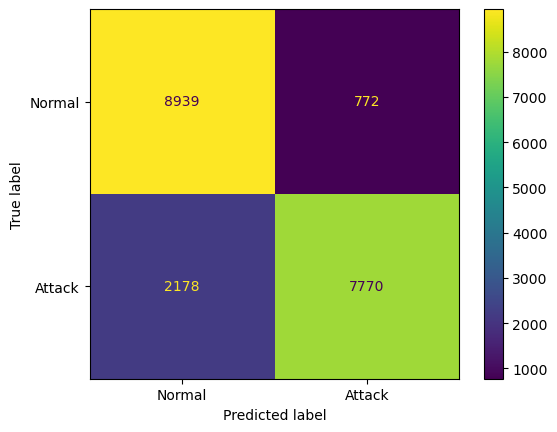
\includegraphics[width=0.7\linewidth]{files/8e5ce1aeec4975bcf56a4273a206e03b.png}

\paragraph{Part 4 - Visualizing}

\subparagraph{Receiver Operating Characteristic (ROC) Curve and Area Under Curve (AUC)}

\begin{verbatim}
from sklearn.metrics import roc_curve, auc
import matplotlib.pyplot as plt

# Generate probabilities
y_pred_prob = classifier.predict(X_test).ravel()

# Calculate ROC curve
fpr, tpr, thresholds = roc_curve(y_test, y_pred_prob)
roc_auc = auc(fpr, tpr)

# Plot ROC curve
plt.figure()
plt.plot(fpr, tpr, label=f'ROC Curve (AUC = {roc_auc:.2f})')
plt.plot([0, 1], [0, 1], 'k - -')  # Random guess line
plt.xlabel('False Positive Rate')
plt.ylabel('True Positive Rate')
plt.title('Receiver Operating Characteristic')
plt.legend(loc='lower right')
plt.savefig('ROC_SC')
plt.show()
\end{verbatim}

\begin{verbatim}
615/615 ━━━━━━━━━━━━━━━━━━━━ 19s 31ms/step
\end{verbatim}

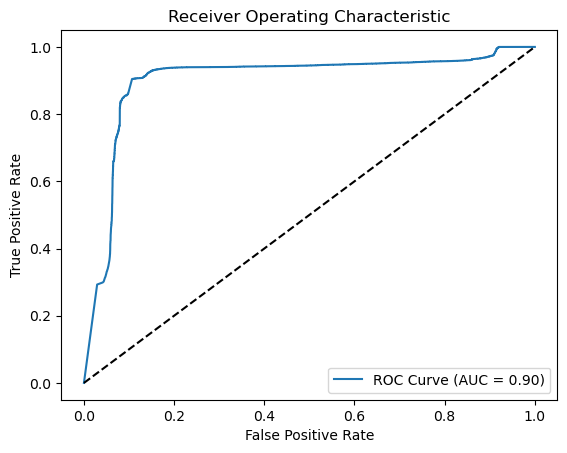
\includegraphics[width=0.7\linewidth]{files/e62ed2afb3ca7bed672153b972465a63.png}

\subparagraph{Plot the accuracy}

\begin{verbatim}
########################################
# Part 4 - Visualizing
#######################################

# Import matplot lib libraries for plotting the figures. 
import matplotlib.pyplot as plt

# You can plot the accuracy
print('Plot the accuracy')
# Keras 2.2.4 recognizes 'acc' and 2.3.1 recognizes 'accuracy'
# use the command python -c 'import keras; print(keras.__version__)' on MAC or Linux to check Keras' version
#plt.plot(classifierHistory.history['accuracy'], label='Training Accuracy')
plt.plot(classifierHistory['accuracy'], label='Training Accuracy')
plt.title('model accuracy')
plt.ylabel('accuracy')
plt.xlabel('epoch')
plt.legend(loc='upper left')
plt.savefig('accuracy_sample_SC.png')
plt.show()
\end{verbatim}

\begin{verbatim}
Plot the accuracy
\end{verbatim}

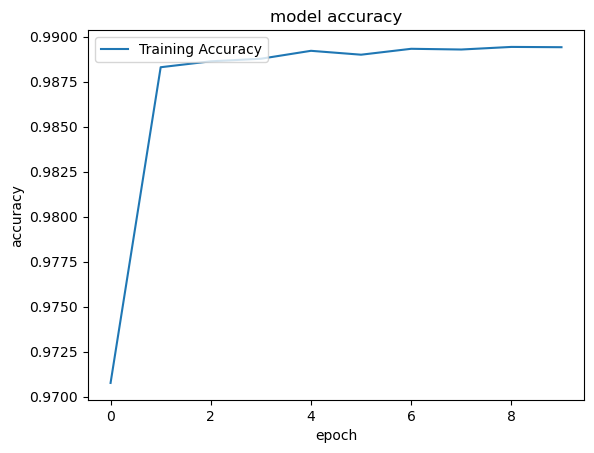
\includegraphics[width=0.7\linewidth]{files/1a46407d56ff032e149c9b079fac1d9a.png}

\subparagraph{Plot the Loss}

\begin{verbatim}
# You can plot history for loss
print('Plot the loss')
#plt.plot(classifierHistory.history['loss'], label='Training Loss')
plt.plot(classifierHistory['loss'], label='Training Loss')
plt.title('model loss')
plt.ylabel('loss')
plt.xlabel('epoch')
plt.legend(loc='upper left')
plt.savefig('loss_sample_SC.png')
plt.show()
\end{verbatim}

\begin{verbatim}
Plot the loss
\end{verbatim}

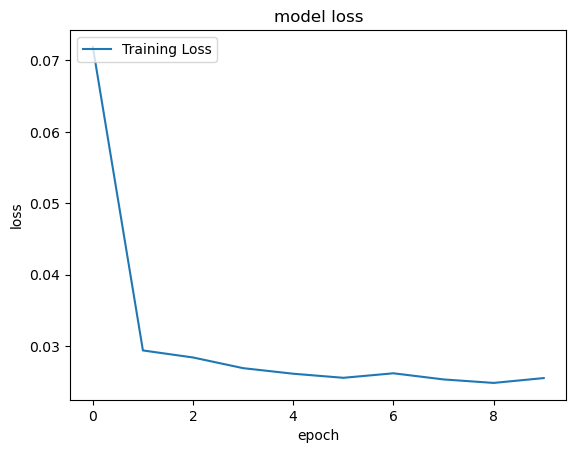
\includegraphics[width=0.7\linewidth]{files/20e5dde01b28f4a3bfea2f230fd6ecf3.png}